% 2. Fragen zur Vorbereitung

\chapter{Theoretischer Hintergrund}
\label{chap:fvz}
Zuerst wollen wir einen auf den theoretischen Hintergrund der Elektronenmikroskope werfen. Dafür wird \citep{RasterEM} und \citep{Anleitung} als Hauptquelle verwendet.
\section{Arten und Vergleich der Mikroskope}
\label{sec:artenEM}
Zur Unterscheidung der einzelnen Mikroskope Arten werden wir diese vorerst aufzählen.

\subsection*{Lichtmikroskop (LM)}
Beim LM werden stark vergrößerte Bilder von kleinen Strukturen oder Objekten mit Hilfe von sichtbaren Licht und optischen System aus Linsen erzeugt.
\begin{itemize}
    \item Auflösung: \SI{0,2}{\micro\metre} $\sim$ \SI{0,3}{\micro\metre}\\
    Wird durch die physikalischen Gesetzmäßigkeiten bestimmt und hängt somit von der Wellenlänge ab. 
    \item Anforderung an Probe: Für gut erkennbare Strukturen im Bild muss die Probe ausreichend Kontrast enthalten \citep{WikiLM}.
\end{itemize}

\subsection*{Transmission-Elektronenmikroskop (TEM)}
Bei einem TEM werden dünne Probe wird mit Elektronen durchstrahlt, welche durch die Streuung ihre Bewegungsrichtung ändern und ihre Energie durch inelastische Stöße verlieren. Die Elektronen, welche das Material durch elastische Stöße unter Erhaltung des Eintrittswinkels verlassen, werden in der hinteren Brennebene fokussiert. Die gestreuten Elektronen werden mit einer Blende abgeschirmt. Entweder wird dann das \textit{Zwischenbild} (vergrößertes Lichtbild) oder das \textit{Elektronenbeugungsbild} (Fokusebene) betrachtet. 
\begin{itemize}
    \item Auflösunggrenze: einige \si{\nano\metre} bis \si{\micro\metre}\\
    Dabei hängt die Auflösung von der Beschleuigungsspannung (80 $\sim$ 400\si{\kilo\volt}) und der Materialdicke ab. 
    \item Anforderung an Probe: Ultradünne Schnitte notwendig (10–\SI{100}{\nano\metre}) \citep{WikiTEM}
\end{itemize}
\newpage
\subsection*{Raster-Elektronenmikroskop (REM)}
Bei einem REM wird durch einen Elektronenstrahl die zu untersuchende Probe zeilenförmig abgerastert. Dabei wird die Topografie (Oberfläche), die Kristallstruktur und Materialunterschiede der Probe auf einen Bildschirm mittels Sekundärelektronen und Rückstoßelektronen (siehe \ref{sec:elektrons}) mit entsprechenden Detektoren abgebildet. Weiterhin lässt ein REM eine Röntgenanalyse zu, wodurch auch eine Elementanalyse der Probe möglich ist.
\begin{itemize}
    \item Auflösung: $\sim$ \SI{10}{\nano\metre}\\
    Das Auflösungvermögen ist dabei von dem Strahlendurchmesser und dem Abbildungsignal abhängig und beträgt zwischen \SI{1}{\nano\metre} $\sim$ \SI{2}{\nano\metre} in günstigen Verhältnissen. \citep{WikiREM}
    \item Eindringtiefe in die Probe: $\sim$ \SI{1}{\micro\metre}
    \item Anforderung an Probe: Vakuumstabil und trocken mit leitender Oberflächenschicht (ggf. aufgetragene Beschichtung)
\end{itemize}
Das REM und seine Funktionsweise wird in weiteren Kapitel noch genauer betrachtet.\\

Die jeweiligen Mikroskope dennoch generelle Vorteile oder Nachteile, die im Folgendem betrachtet werden.
\subsection*{(REM,TEM) vs LM}
\begin{itemize}
    \item[\textcolor{green}{\textbf{+}}] Licht mit viel größerer Wellenlänge (\SI{380}{\nano\metre}) als Elektronen (Welle-Teilchen-Dualismus)(de-Broglie: \SI{5}{\nano\metre}) $\Rightarrow$ Erheblich bessere Auflösung
    \item[\textcolor{red}{\textbf{-}}] (REM,TEM) benötigt Vakuum im Gang des Elektronenstrahl und elektromagnetische Linsen, während eine LM \enquote{nur} Glaslinsen benötigt $\Rightarrow$ Höherer technischer Aufwand \citep{RuppelEM}
\end{itemize}

\subsection*{REM vs TEM}
\begin{itemize}
    \item[\textcolor{green}{\textbf{+}}] Probenpräparation einfacher, da keine ultradünnen Schnitte der Probe erzeugt werden müssen
    \item[\textcolor{green}{\textbf{+}}] 3D-Abbildung der Oberfläche des Objekts $\Rightarrow$ leicht verständliche Bilder 
    \item[\textcolor{red}{\textbf{-}}] geringere Vergrößerung und Auflösung
    \item[\textcolor{red}{\textbf{-}}] Keine Aussage über innere Struktur der Probe \citep{RuppelEM} 
\end{itemize}
\newpage
\section{Aufbau eines Raster-Elektronenmikroskops}
\label{sec:aufbau}
In diesem Versuch ist vor allem das Rasterelektronenmikroskop von besonderem Interesse. Dessen Aufbau wird in \ref{image:aufbau} dargestellt. 
In einer Mikroskopsäule durch eine thermische Wolframkathode (Elektronenquelle), welche von einem Wehnelt-Zylinder umschlossen ist, eine Elektronenwolke erzeugt. Diese Elektronenwolke wird durch eine Crossover Anode nach unten beschleunigt und wird durch die Kondensorlinsen (Elektronenlinsen) zu einem Elektronenstrahl fokussiert. Die Stigmatoren verhindern dabei, dass ein \textit{axialer Astigmatismus} in der Abbildung auftritt. Der Durchmesser des Elektronenstrahls wird dann weiter nach unten durch die Kondensorlinsen und der Aparturblende (\SI{50}{\milli\metre}) elektronenoptisch verkleinert. Ablenkspulen sorgen dann für zeilenförmigen Abrasterung der Probe durch den Elektronenstrahl. Die verschiedenen Elektronen werden dann von einem Everheart-Thornley-Detektor und Halbleiterdetektor registriert und die entstehende Röngtenstrahlung von einem EDX-Detektor (siehe \ref{sec:detect}). Dabei dienen die registrierten Elektronen als Signal zur Helligkeitsmodulation des Bildes.
\begin{center}
    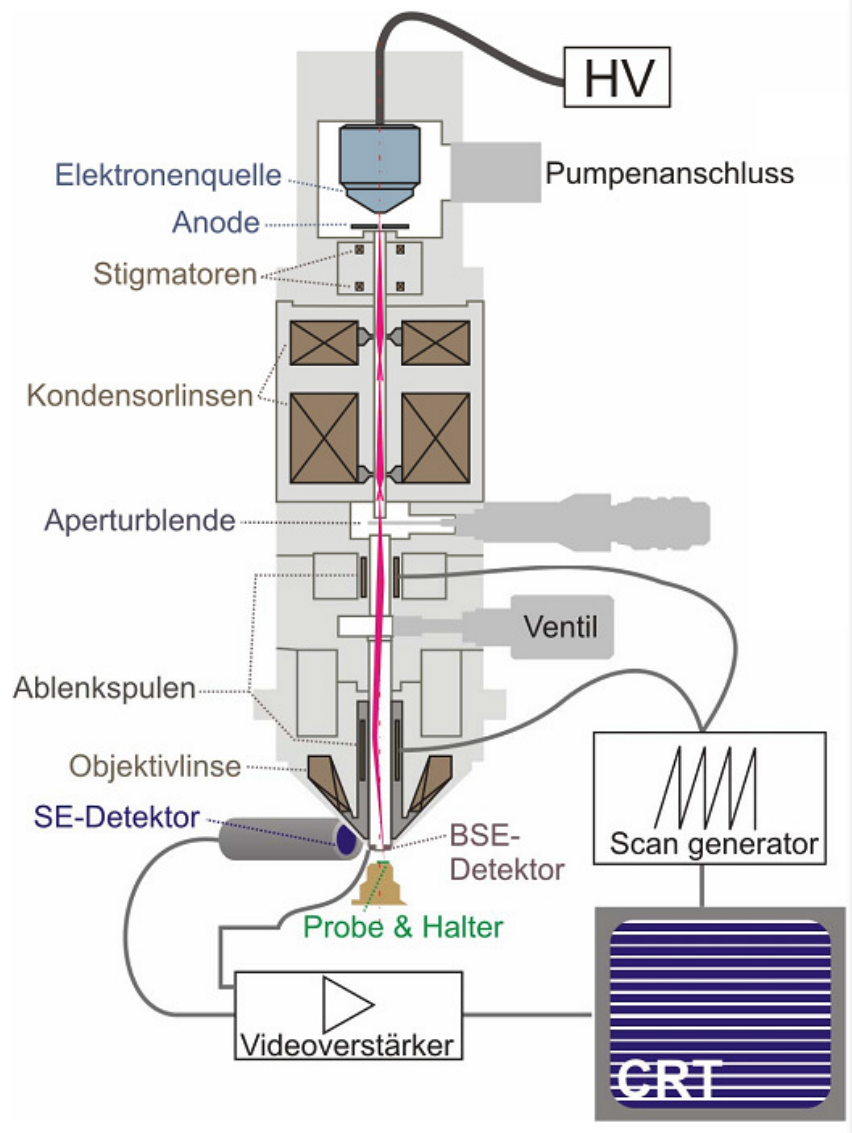
\includegraphics[scale=0.25]{AufbauREM.png}
    \captionof{figure}{Aufbau Raster-Elektronenmikroskop \citep{Anleitung}}
    \label{image:aufbau}
\end{center}
Eine weitere wichtige Größe eines REM ist die \textit{\textbf{Schärfentiefe}}. Die Schärfentiefe ist ein Maß, welches angibt in welchen Bereich oberhalb und unterhalb die Probe noch Scharf aufgelöst werden kann.  Diese hängt von der Größe der Apertur und dem Arbeitsabstand ab. Dabei gilt eine kleine Blende und ein großer Arbeitsabstand besitzen eine hohe Schärfentiefe. 
%\begin{center}
%    \begin{tabular}{cc}
%        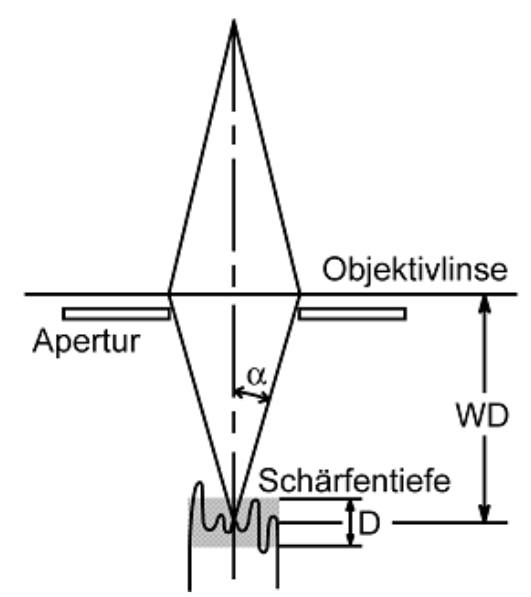
\includegraphics[scale=0.2]{Schaerfentiefe1.png} & 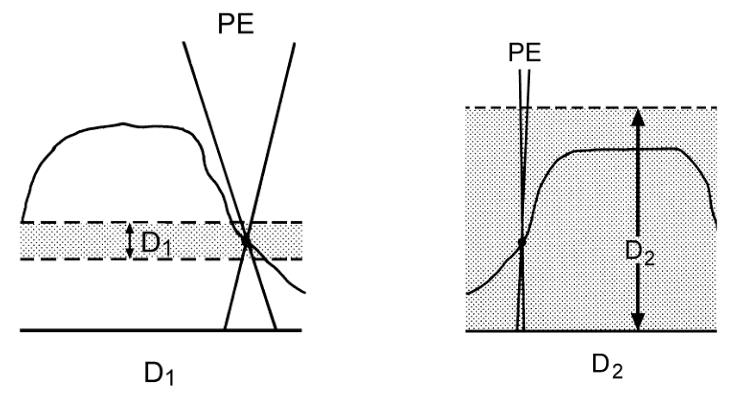
\includegraphics[scale=0.2]{Schaerfentiefe2.png}
%    \end{tabular}
%    \captionof{figure}{Schärfentiefe \citep{Anleitung}}
%\end{center}

\section{Wechselwirkung der Elektronen mit Materie}
\label{sec:elektrons}
Durch Wechselwirkung des Primärelektronenstrahls (PES) (mit Primärelektronen (PE)) mit der Probe entstehen unterschiedliche Signale. In Abb. \ref{image:signal} wird schematisch dargestellt wie der PE mit der Probe reagiert. Dabei werden unterschiedliche Arten von Signalen erzeugt: Elektronensignal und Röntgenstrahlung sowie Lumineszenz. Für die Analyse des Stoffes ist nur die Röntgenstrahlung von Interesse, während das Elektronensignal für die Abbildung verantwortlich ist. Die Elektronen, welche von der Probe absorbiert werden, erzeugen einen Probenstrom, welcher über die Erde abgeleitet wird. 
\begin{center}
    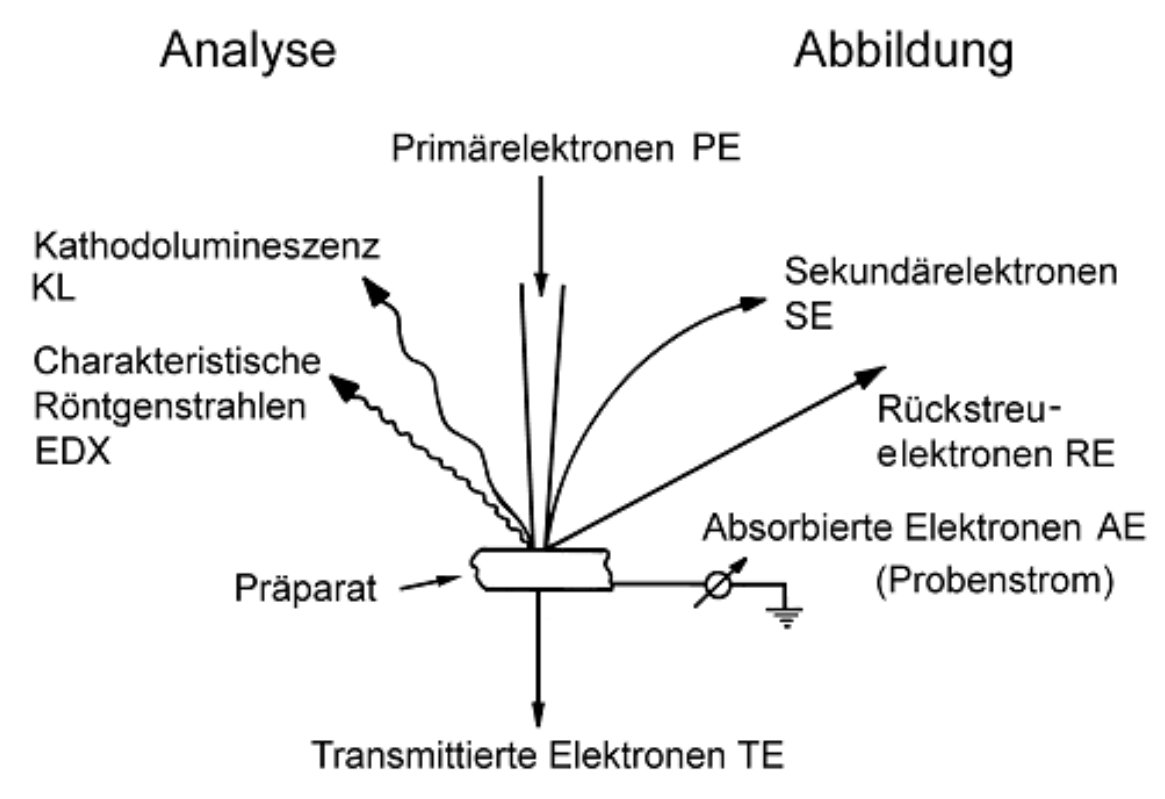
\includegraphics[scale=0.2]{Signalentstehung.png}
    \captionof{figure}{Signale eines REMs \citep{Anleitung}}
    \label{image:signal}
\end{center}
Das Volumen, in dem die Elektronen des Primärelektronenstrahls (PES) mit dem Atomkernen der Probe wechselwirken, wird Streubirne oder Elektronendiffusionswolke genannt, wobei die Reichweite gewählten Anregungsspannung abhängt. 
\begin{center}
    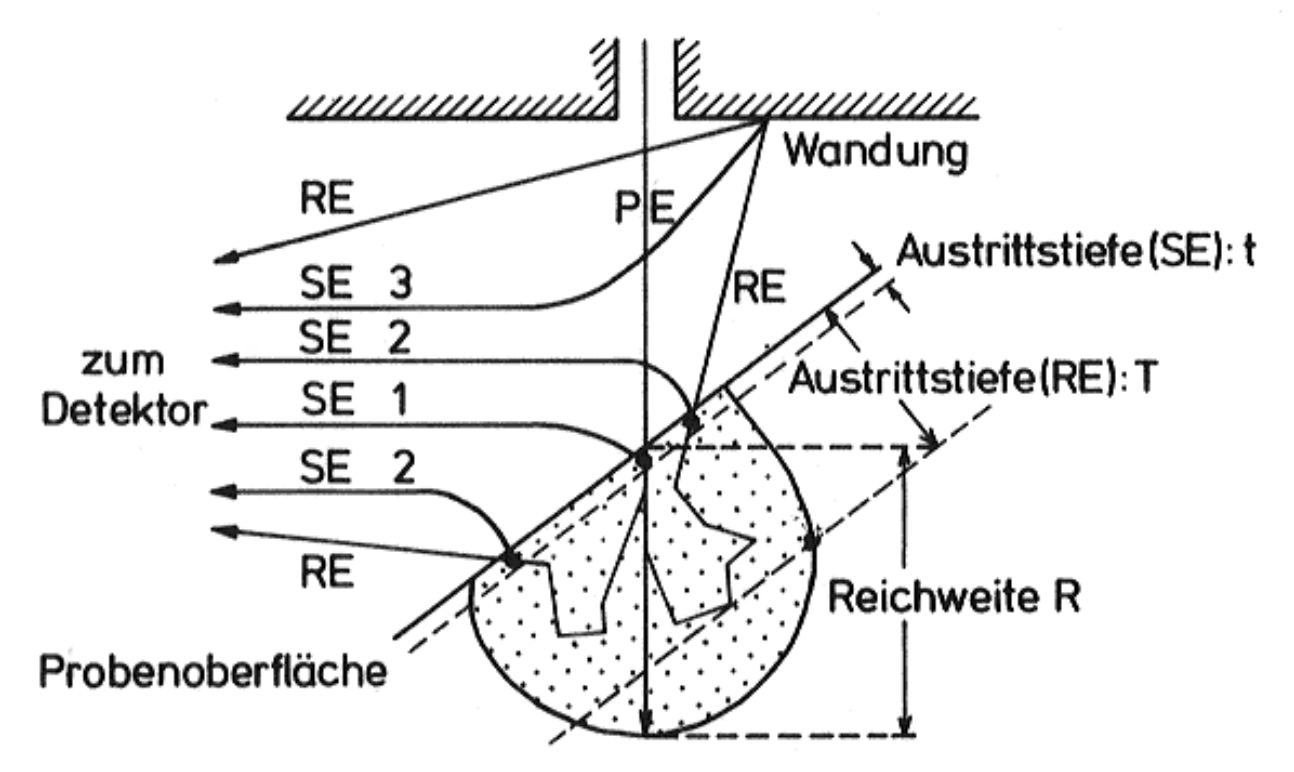
\includegraphics[scale=0.17]{Elektronendiffusionswolke.png}
    \captionof{figure}{Elektronendiffusionswolke \citep{RasterEM}}
    \label{image:wolke}
\end{center}
\newpage
\section*{Elektronensignal}
PE, welche elastisch an Atomkerne in der Probe gestreut werden und diesen unter großen Winkel verlassen, werden als \textbf{\textit{Rückstreuelektronen (RE)}}. RE haben dabei eine Ernergie $E > \SI{50}{\electronvolt}$, worunter auch schnellere SE fallen, aber diese sind von RE nicht unterscheidbar. Die ausgelösten RE stammen dabei aus einer Materialtiefe $T=$0,1-\SI{1}{\micro\metre} (siehe Abb. \ref{image:wolke}). Auch hängt die Ausbeute der RE von der Kernladungszahl des Materials ab \citep{WikipolyREM}.\\
Weiterhin entsteht durch unelastische Streuung der PE langsame \textbf{\textit{Sekundärelektronen (SE)}} mit Energie $E < \SI{50}{\electronvolt}$ und mit wahrscheinlichster Energie $\left\langle E\right\rangle=1-\SI{5}{\electronvolt}$, welche aus der Tiefe $t =$ 1-\SI{10}{\nano\metre} (siehe Abb. \ref{image:wolke}) stammen und zur Hochauflösung des REM führen.\\
Die SE werden dann in Gruppen unterteilt:
\begin{itemize}
    \item \textbf{SE 1:} Durch PE im Material erzeugte SE
    \item \textbf{SE 2:} Durch RE im Material erzeugte SE 
    \item \textbf{SE 3:} Durch RE außerhalb des Materials erzeugte SE\\   
\end{itemize}
Der Vorgang der Erzeugung unterschiedlicher SE ist in Abbildung \ref{image:wolke} dargestellt. Aufgrund der unterschiedlichen Energien der SE und RE (siehe Abb. \ref{image:energieverteilung}) kann man mit der richtigen Einstellung des Detektors die Art des Signals steuern, was später behandelt wird.
\begin{SCfigure}[][h]
    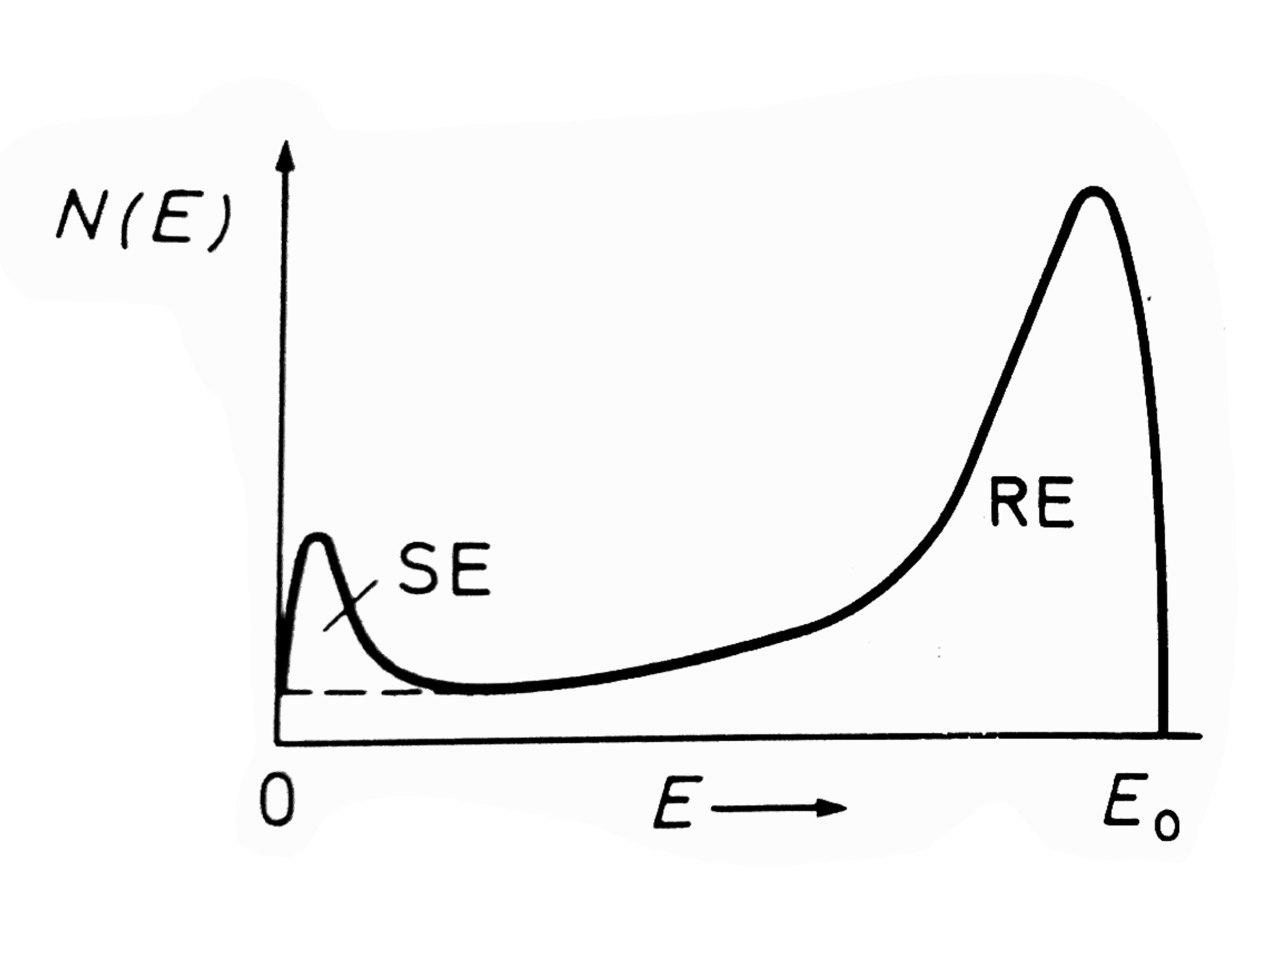
\includegraphics[scale=0.10]{Energieverteilung.jpg}
    \caption{Schematische Energieverteilung der Anzahl von SE und RE bei normierter Energie \citep{RasterEM}}
    \label{image:energieverteilung}
\end{SCfigure}
\section*{Röntgenstrahlung}
Bis zu einer Reichweite von $R=\SI{500}{\nano\metre}$ (siehe Abb. \ref{image:wolke}) entsteht eine Wechselwirkung des PES mit der Probe, wobei Elektronen aus der Atomhülle geschlagen werden. Elektronen aus höheren Zuständen können auf niedrigen Zustand herunterfallen und es entsteht Röntgenstrahlung. Diese Strahlung ist charakteristisch für das jeweilige Element.\\Die emittierende Strahlung kann dann noch ein Elektron aus einer höheren Schale herausschlagen, was als Auger-Elektron registriert wird. Bei Kernen mit kleiner Ordnungszahl ($Z$<20) dominiert die Emission von Auger-Elektronen, bei höheren Ordnungszahlen überwiegt die Emission von charakteristischer Röntgenstrahlung.\\

Weiterhin entsteht auch durch das Abbremsen von Elektron am Atomkern in der Probe das sogenannte Bremsspektrum. Bei diesem Vorgang gibt das Elektron die überschüssige Energie in Form von Strahlung ab. Das Bremsspektrum und die Röntgenstrahlung der Elektronen-Übergänge ergeben dann das charakteristische Röntgenspektrum.
\newpage
\section{Detektoren}
\label{sec:detect}
Das Rasterelektronenmikroskop besitzt mehrere Detektoren, mit denen es möglich ist die unterschiedlichen zuvor besprochenen Signale zu verarbeiten. Hierfür sehen wir uns zuerst die Detektoren für die Elektronensignale und dann die für die Röntgenstrahlung an.  
\subsection{Elektronendetektoren}
\subsection*{Everheart-Thornley-Detektor}
\label{sub:etDetect}
\begin{center}
    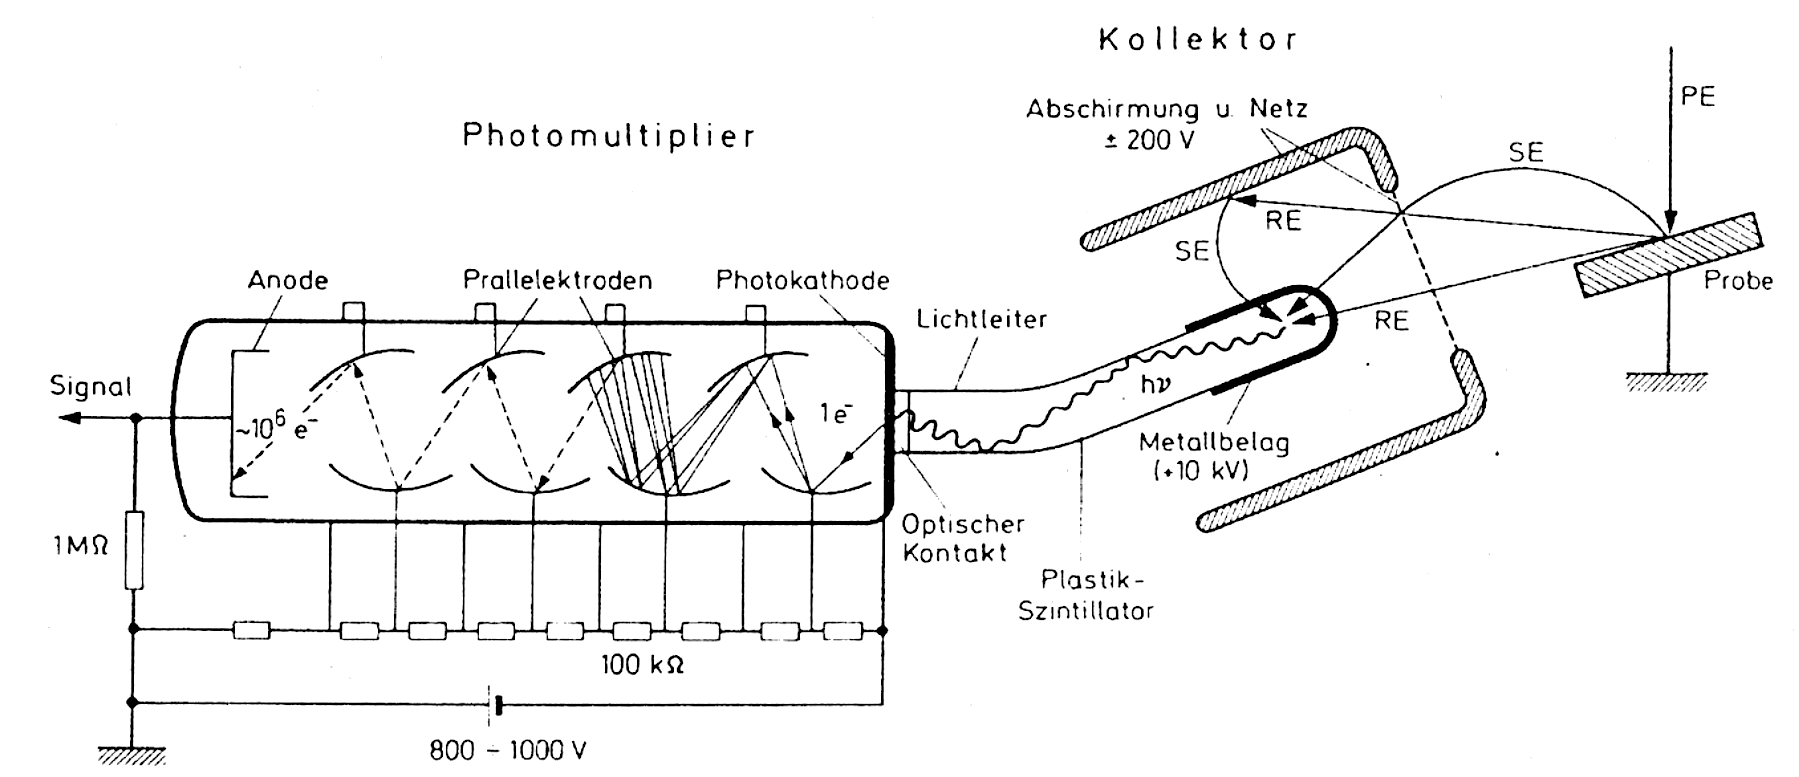
\includegraphics[scale=0.18]{Everheart-Thornley.png}
    \captionof{figure}{Everheart-Thornley-Detektor \citep{RasterEM}}
    \label{image:etDetect}
\end{center}
Der Everheart-Thornley-Detektor ist eine Kombination aus Szintillator und Photomultiplier (siehe Abb. \ref{image:etDetect}). Dieser dient zur Detektierung von SE und RE. Die aus er Probe gelösten SE werden dabei von einem Netz des Kollektors mit positiver Spannung angesaugt (mit negativer Spannung können SE zurückgehalten werden $\Rightarrow$ nur RE im Signal). Schnelle RE, welche einen wesentlich höhere Energie wie SE haben, passieren das Netz in beiden Fällen. Auf einer \SI{50}{\nano\metre} dünnen, leitende Metallschicht auf der Oberfläche des Plastik-Szintillators liegt eine Spannung von \SI{10} {\kilo\volt}, welche die Elektronen vom Netz zum Szintillator beschleunigen. Dabei entstehen im Szintillator eine große Elektron-Loch-Paar, welcher proportional zur Spannung zwischen Probe und Kollektor und der Neigung der Probe zum Kollektor ist. Die Rekombination dieser Paare erzeugt Lichtquanten, wobei ein großer Teil strahlungslos rekombiniert. Dabei werden die erzeugten Photonen durch Totalreflexion in Richtung des Photomultiplier abgelenkt. Auf der Photokathode wird dann durch das Photon ein Elektron ausgelöst, wobei diese durch mehrere Prallelektrode auf \SI{100}{\electronvolt} beschleunigt und Spannungsimpulse induzieren, welche wiederum elektronisch verstärkt werden können. Dabei führt jedes einfallende SE mindestens zu einem Spannungsimpuls. Die Spannungsimpuls sorgen dann für einen Steuerung der Bildschirmhelligkeit.
\newpage
\subsection*{Halbleiterdetektor}
\label{sub:halbDetect}
\begin{center}
    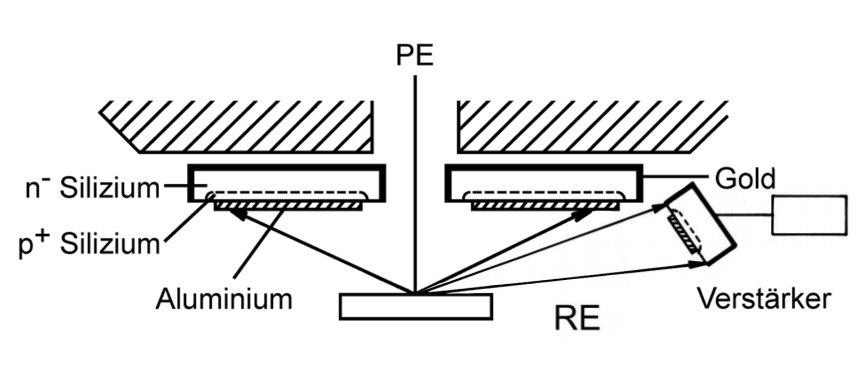
\includegraphics[scale=0.3]{Halbleiterdetektor.jpg}
    \captionof{figure}{Halbleiterdetektor \citep{Anleitung}}
    \label{image:halbDetect}
\end{center}
Halbleiterdetektor sind im Grunde Dioden, welche in Sperrrichtung betrieben werden. Dafür eigenen sich diese Detektoren besonders gut für die Untersuchung von REs. Durch das Aluminium, welches vor dem Halbleiter montiert ist (siehe Abb. \ref{image:halbDetect}), wird verhindert, dass emittiere Lichtquanten von der Probe mitdetektiert werden. Auch werden langsame SEs von der Al-Schicht absorbiert. Die RE erzeugen im Leiter Elektron-Loch-Paare, welche dann über den p-n-Übergang diffundieren können, wobei es dort zu Rekombinationen in der jeweiligen Schicht kommt oder diese auch getrennt werden. Durch die Trennung der Elektron-Loch-Paare fließt durch den Leiter ein Strom, welcher weiter verstärkt wird und wiederum zur Helligkeitsmodulation dient. Durch seine flache Bauform kann der Halbleiterdetektor nahe an der Probe angebracht werden und erlaubt damit im Gegensatz zum Everheart-Thornley-Detektor die Abbildung eines großen Raumwinkels.
\begin{center}
    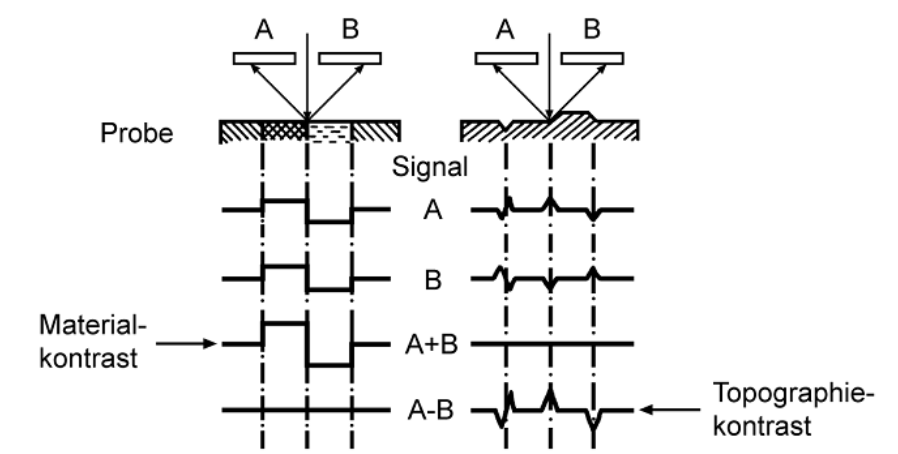
\includegraphics[scale=0.3]{Modi.png}
    \captionof{figure}{Compo- und Topomode \citep{RasterEM}}
    \label{image:modi}
\end{center}
Der Halbleiterdetektor kann in verschiedenen Modi betrieben werden (siehe Abb. \ref{image:modi}). Den Compo- (Materialkontrast) und den Topo-Mode (Topografiekontrast).
Weiterhin kann das verwendete Elektronenmikroskop in Praktikum den sogenannten Shadow-Mode, welcher es ermöglicht Compo- und Topo-Mode gleichzeitig darzustellen. Möglich gemacht wird dies mit Hilfe es dritten Detektor, welcher leicht schräg angewinkelt ist (siehe Abb. \ref{image:halbDetect}).
\subsection{Röntgendetektoren}
\subsection*{Si(Li)-Detektor und SDD-Detektor (Jetzt: Xray-Detektor)}
\label{sub:siliDetect}
Bei einem Si-Detektor handelt es sich im Grunde um eine in Sperrrichtung betriebenen Silizium-Diode. Dabei wird bei einer angelegten Sperrspannung eine ladungsträgerfreie Zone(intrinsische Zone) erzeugt. Durch die einfallenden Röntgenquanten werden Elektron-Loch-Paare erzeugt, die durch die angelegte Sperrspannung zu den Elektroden getrennt werden und dabei einen Spannungsimpuls verursachen. Für höhere Effizienz wird die Si-Diode mit Lithium dotiert, womit der Si(Li)-Detektor entsteht. Das Lithium fungiert als Donator und erzeugt mit den p-leitenden Charakter des Siliziums einen p-i-n-Übergang. Um das Driften der Lithium-Ionen zu verhindern, muss der Si(Li)-Detektor permanent gekühlt werden.
\begin{center}
    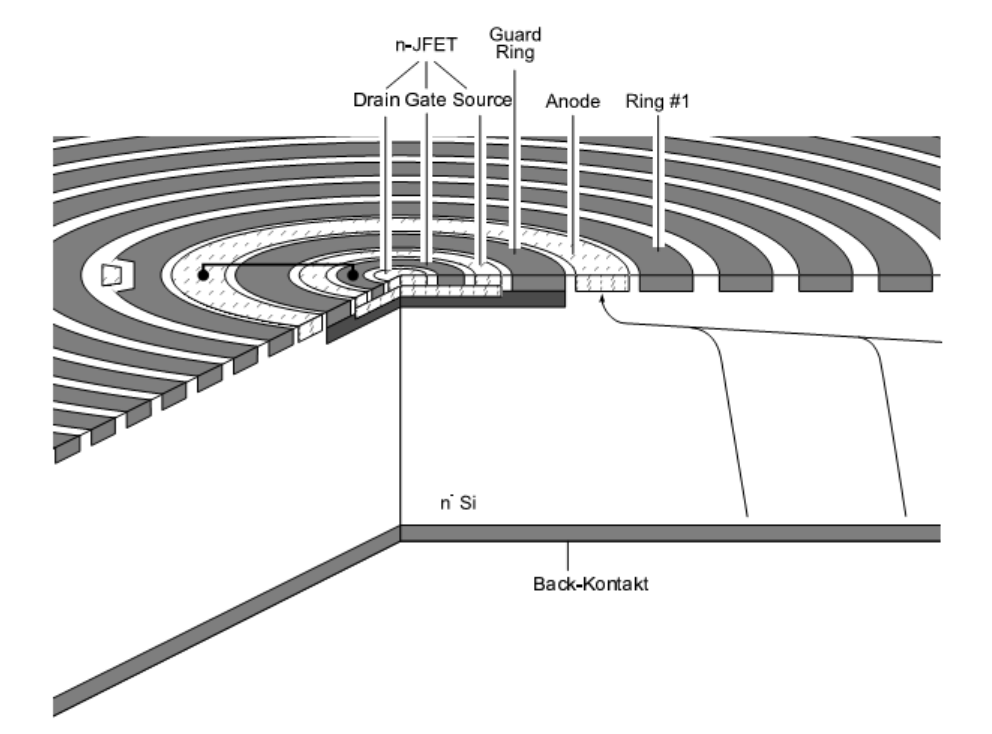
\includegraphics[scale=0.17]{Wafer.png}
    \captionof{figure}{SDD-Detektor \citep{Anleitung}}
    \label{image:sddDetect}
\end{center}
Ein Silizium Drift Detektor (SDD) besteht nur aus einem Silizium-Wafer, der mit ringförmigen Elektroden auf der obereren Seite besitzt. Hierbei weist die angelegte Spannung einen Gradienten auf, welcher von Innen nach Außen zunimmt. Als Signalverstärker fungiert ein Feldeffekt Transistor (FET) im Zentrum des Wafers. Der SDD besitzt dabei keine klassische Diodenstruktur und besteht dabei aus zwei gegenüberliegenden p+ dotierten Schichten mit n- dotierter Rückseite als Sammelelektrode. Bei Sperrspannung entsteht auch wieder eine ladungsträgerfreie Zone und ein Potenzialminimum im Zentrum des Wafers, wobei somit ein Spannungsgradient erzeugt wird, der die Elektronen (aus Elektron-Loch-Paar erzeugt durch Röntgenquant) zur Anode leitet und die Löcher zu den Driftringe (siehe Abb. \ref{image:drift}).
\begin{center}
    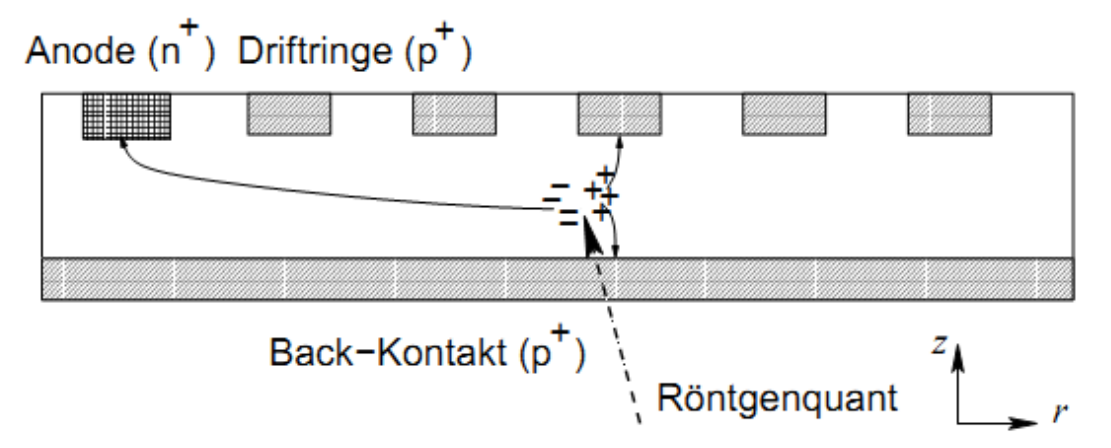
\includegraphics[scale=0.2]{WaferFunk.png}
    \captionof{figure}{Driftfeld SDD-Detektor \citep{Anleitung}}
    \label{image:drift}
\end{center}
Der SDD nimmt dabei das klassische Röntgenspektrum (siehe Kapitel \ref{sec:elektrons})) auf, wobei die $K_\alpha$ für die praktische Analyse am wichtigsten ist, da diese am wahrscheinlichsten entsteht. Die Aufnahme der Spektrallinien kann wellenlängendispersiv oder energiedispersiv erfolgen. Bei einem wellenlängendispersiven Spektrometer (WDS) werden jeweils auf eine Spektrallinie (mit Hilfe eines Analysatorkristall) direkt eingestellt, wodurch eine genaue Bestimmung der Intensität möglich ist. Bei einem energiedispersiven Spektrometer (EDS) wird simultan das gesamte Röntgenspektrum erfasst wird, was eine gute Übersicht über die auftretenden Linien gibt. Wichtig zu erwähnen ist, dass ein EDS auch bei rauhen Oberflächen ohne Intensitätsabnahme verwendet werden kann, wobei die Messung nur qualitativ ist. Auch ist zu beachten, dass bei einem EDS Überlappungen auftreten können. Speziell die M- und L-Linien höherer Ordnungszahlen mit der mit den K-Linien niedrigen Ordnungszahlen können sich Überlappen.\\

In Abbildung \ref{image:jeolDetect} ist die Anordnung der Detektoren im Jeol JSM 6510 abfotografiert um einen Eindruck für das Aussehen der Detektoren zu schaffen.
\begin{center}
    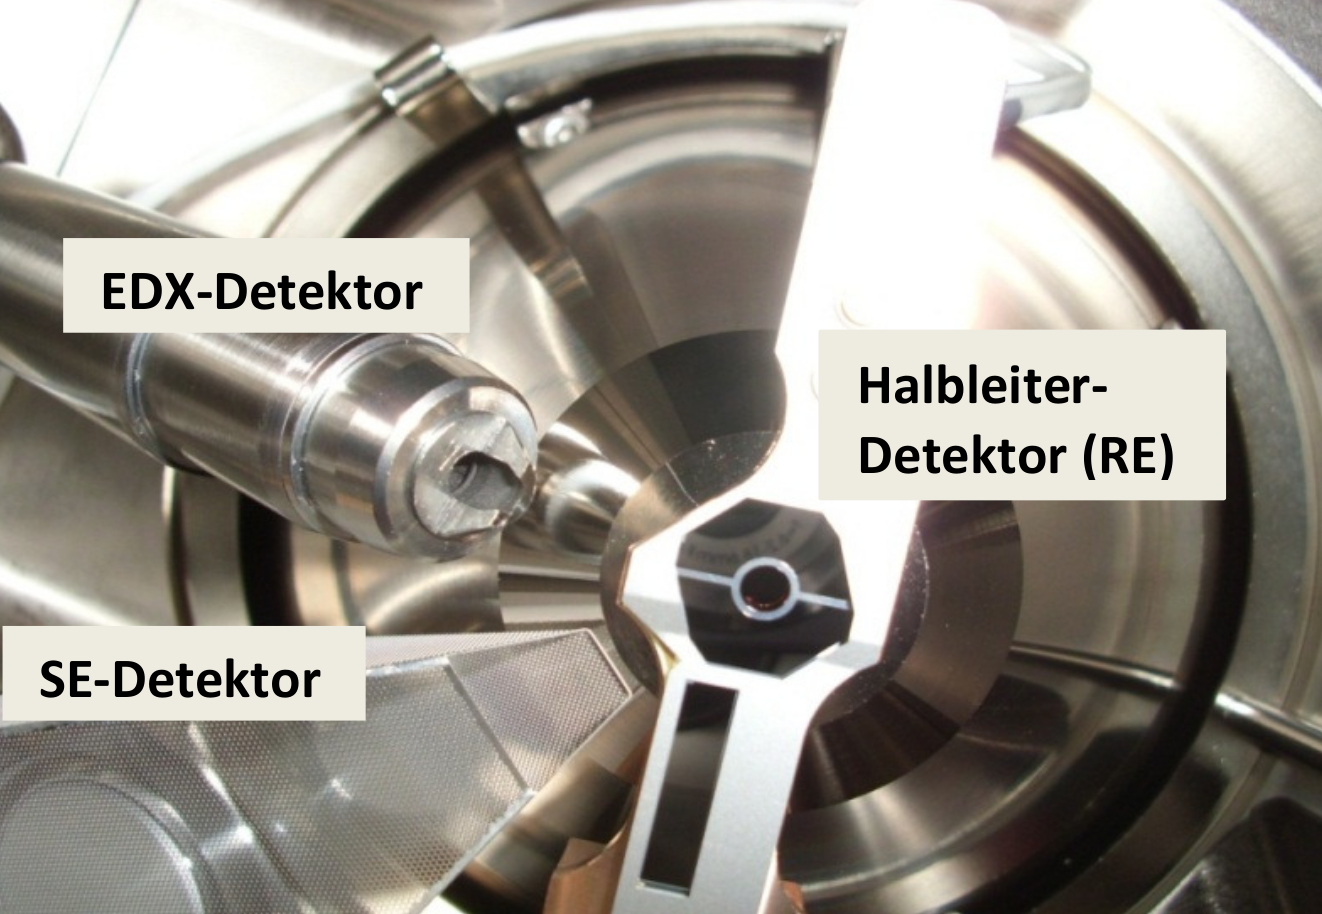
\includegraphics[scale=0.2]{Detektoren.png}
    \captionof{figure}{Detektoren bei Jeol JSM 6510 \citep{Anleitung}}
    \label{image:jeolDetect}
\end{center}
\newpage
\section{Linsenfehler}
\label{sec:linError}

Bei einem Elektronenmikroskop können auch aufgrund des Welle-Teilchen-Dualismus des Elektrons die bekannten Linsenfehler aus der Optik auftreten. Dabei gibt es folgende Linsenfehler:
\begin{itemize}
    \item[\textbf{1)}]\textbf{Öffnungsfehler:}\\
    Starke Ablenkung und geringere Brennweite bei Strahlen, die in einem großen Abstand von der Achse einfallen. Dabei tretet statt des Brennpunkts ein Kreis mit kleinen Durchmesser auf und der Fehler nimmt mit wachsendem Arbeitsabstand zu (siehe Abb. \ref{image:linError}a). 
    \item[\textbf{2)}]\textbf{Farbfehler (Chromatische Fehler):}\\
    Brennweitendifferenz bei verschiedenen Wellenlängen, wobei dabei ein Zerstreuungskreis entsteht. Durch Stabilisierung der Beschleuigungsspannung und Linsenströme muss dieser Fehler nicht berücksichtigt werden (siehe Abb. \ref{image:linError}b).
    \item[\textbf{3)}]\textbf{Axialer Astigmatismus:}\\
    Durch Fehler in den Elektronenlinsen und der Apperaturblende kann die Brennweite zweier aufeinander senkrecht stehenden ebenen Elektronenbündel eine unterschiedliche Größe haben (siehe Abb. \ref{image:linError}c). Dabei kann der Astigmatismus als Wirkung einer überlagerten Zylinderlinse aufgefasst werden, welcher durch eine zusätzliche senkrechte Zylinderlinse (Stigmator siehe Kapitel \ref{sec:aufbau}) korrigiert werden kann. 
    \item[\textbf{4)}]\textbf{Beugungsfehler:}\\
    Aufgrund Apperaturbegrenzung ist der Fokus nicht scharf, wodurch an einem Punkt neben dem Fokus Interferenzen entstehen und damit ein Beugungsbild (siehe Abb. \ref{image:linError}d).
    \item[\textbf{5)}]\textbf{Zusätzliche Fehler:}\\
    Koma-, Verzeichnung- oder nichtaxiale Farbfehler werden durch kleine Aperturen und Zentrierung des Gerätes korrigiert. 
\end{itemize}
\newpage
\begin{center}
    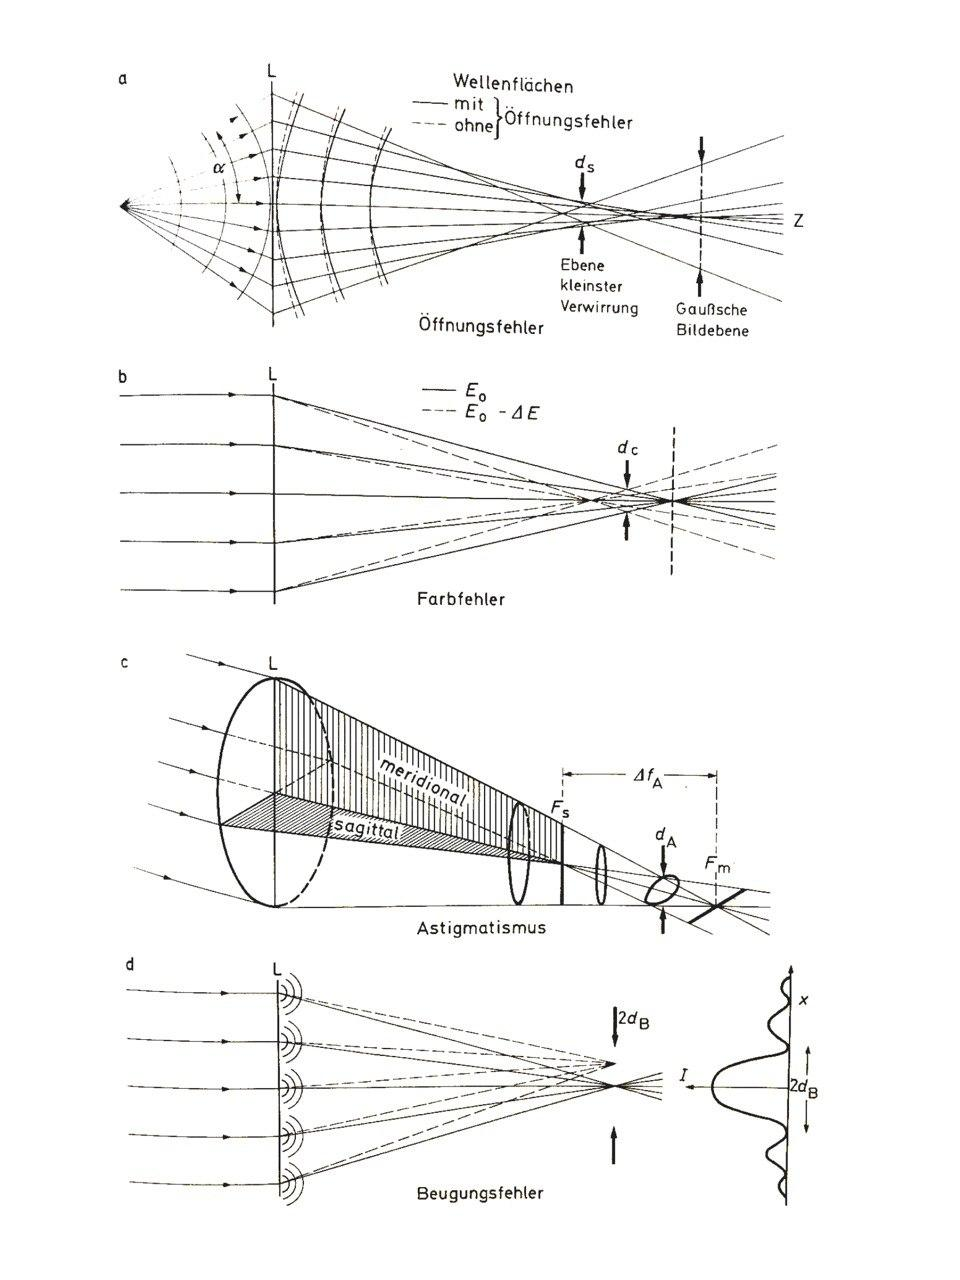
\includegraphics[scale=0.43]{Abbildungsfehler.jpg}
    \captionof{figure}{Linsenfehler \citep{RasterEM}}
    \label{image:linError}
\end{center}

\section{Kontraste}
\label{sec:kontrast}
Die Aufnahme der Bilder des REM erscheinen je nach Kontrast an bestimmten Stellen heller oder dunkler. Diese Kontraste sind sehr wichtig bei der Analyse solcher Bilder, weswegen wir diese nun in folgenden besprechen.
\begin{itemize}
    \item[(1)]\textbf{Topografiekontrast}\\
    Die ausgelösten SE stammen wie vorher besprochen aus der oberen Schicht der Probe, womit die SE die Oberfläche der Probe wiedergibt. Je nach Ausbeute der SE können Flächen heller oder dunkler erscheinen, was den Topografiekontrast der Probe darstellt.
    \item[(2)]\textbf{Flächenneigungskontrast}\\
    Flächenneigungskontraste entstehen durch die Neigung der Probe hin zum Detektor (hier Everhart-Thornley), wodurch die Ausbeute der SE erhöht wird. Durch die Neigung wird die Streubirne (Abb \ref{image:wolke}) abgeschnitten, was zu einer Erhöhung der Fläche, aus welcher die SE treten können, führt. Diese Flächen erscheinen dann im Bild heller als die Flächen vom Detektor weggeneigt. In Abb. \ref{image:neigKontrast} zeigt hierbei die Entstehung und Aussehen des Flächenneigungskontrasts.
    \begin{center}
        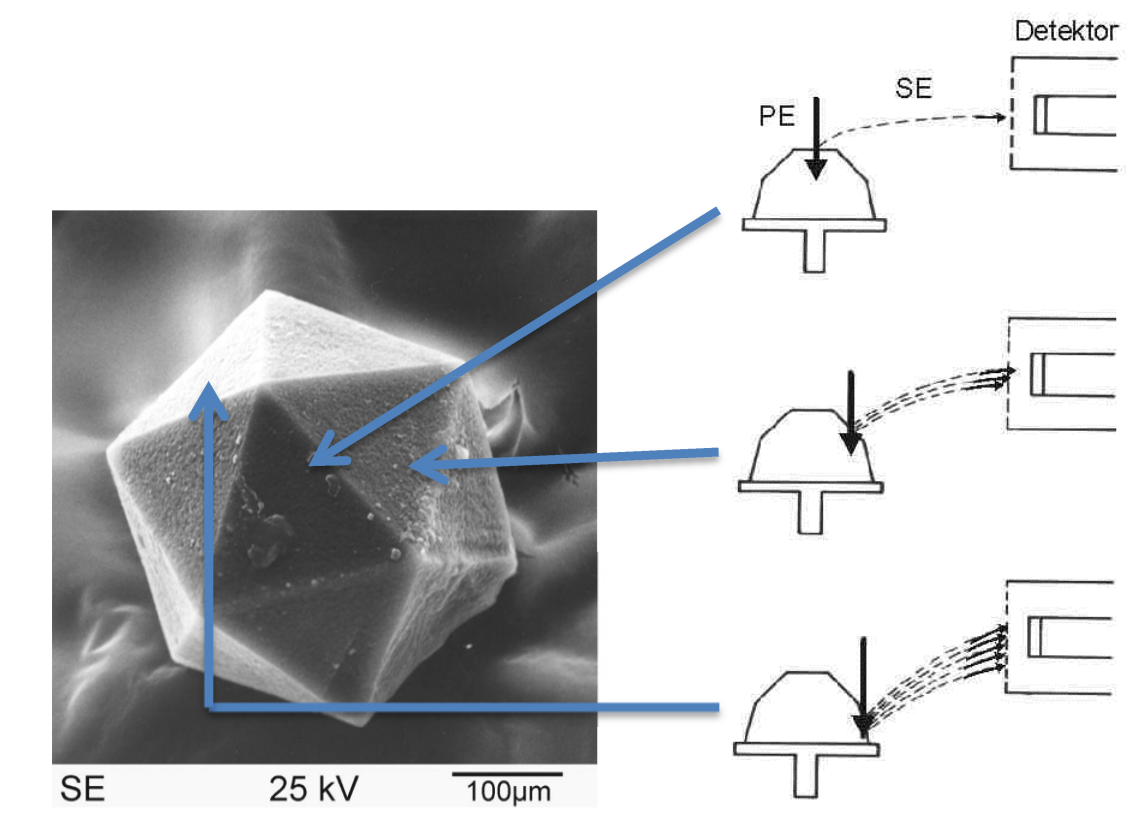
\includegraphics[scale=0.3]{flaechenneigung.png}
        \captionof{figure}{Darstellung Flächenneigungskontrast \citep{Anleitung}}
        \label{image:neigKontrast}
    \end{center}
    \item[(3)]\textbf{Kanteneffekt}\\
    Wie in Kapitel \ref{sec:elektrons} erwähnt können RE bei ihrem Austritt aus dem Material SE auslösen. Dies tritt sehr stark an Kanten auf, da dort mehr RE die Probe verlassen können (siehe Abb. \ref{image:kantKontrast}). Dabei bewirkt der Kanteneffekt, dass die genaue Form der Kante sehr schlecht zu erkennen ist. Vermieden werden kann dies, indem die Primärenergie des Elektronenstrahls herabgesetzt wird.
    \begin{center}
        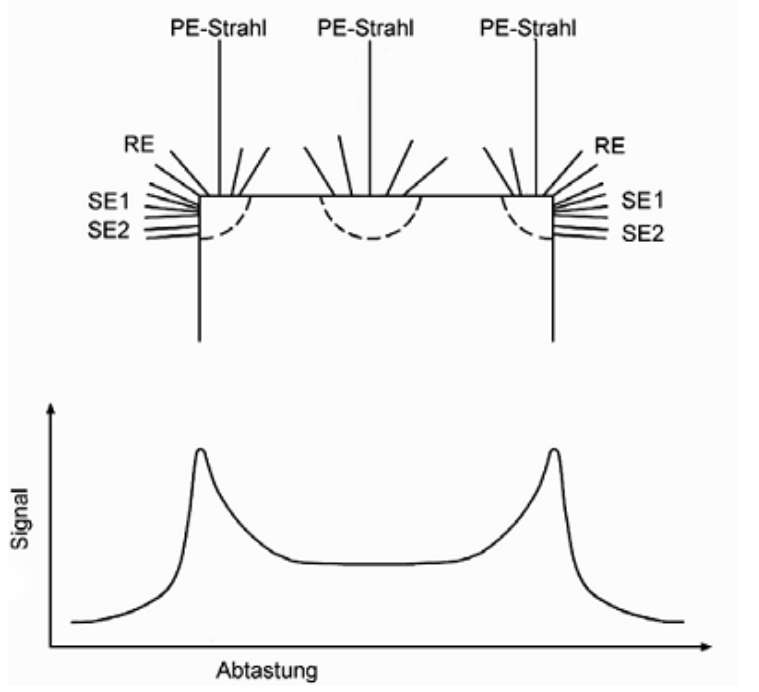
\includegraphics[scale=0.3]{Kanten.png}
        \captionof{figure}{Kanteneffekt und Intensitätsverteilung \citep{Anleitung}}
        \label{image:kantKontrast}
    \end{center}
    \item[(4)]\textbf{Abschattungskontrast}\\
    Im Schatten der Probe können ausgelöste RE und SE den jeweiligen Detektor nicht erreichen. RE, welche auf gradlinigen Bahnen zum Detektor gelangen können, erzeugen sehr scharfe Schattenkanten (siehe Abb. \ref{iamge:schattKontrast}). Schwache Untergrundintensität im Schatten entstehen durch doppelten Rückstreuung der Elektronen an den Probenkammerwänden.
    \begin{center}
        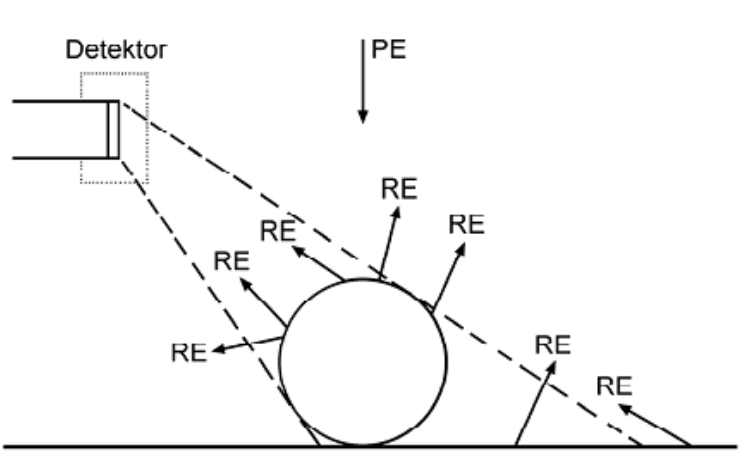
\includegraphics[scale=0.3]{Abschattung.png}
        \captionof{figure}{Entstehung Abschattenungskontrast \citep{Anleitung}}
        \label{iamge:schattKontrast}
    \end{center}
    \newpage
    \item[(5)]\textbf{Materialkontrast}\\
    Der Materialkontrast entsteht durch RE, wodurch Material unterschiedlich hell im Bild erscheinen. Dabei ist die Streuung der RE abhängig von der Kernladungszahl $Z$ (siehe Abb. \ref{image:matKontrast}). Bei höheren $Z$ ist auch der Materialkontrast höher. Wichtig ist dabei, dass die Fläche eben und der Compomodus (Kapitel \ref{sub:halbDetect}) aktiviert ist.
    \begin{center}
        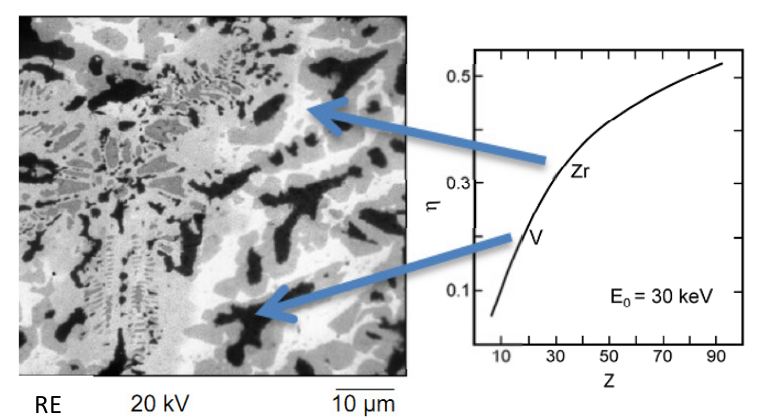
\includegraphics[scale=0.3]{Material.png}
        \captionof{figure}{Materialkontrast in Abhängigkeit der Ordnungszahl}
        \label{image:matKontrast}
    \end{center}
\end{itemize}